% Created 2019-01-06 Sun 23:43
% Intended LaTeX compiler: pdflatex

\documentclass[12pt,a4paper]{article}
\usepackage[margin=2cm]{geometry}
\usepackage{fontspec}
\setromanfont{cwTeXMing}
\usepackage{etoolbox}  % Quote 部份的字型設定
\newfontfamily\quotefont{cwTeXFangSong}
\AtBeginEnvironment{quote}{\quotefont\small}
\setmonofont[Scale=0.9]{Courier} % 等寬字型 [FIXME] Courier 中文會爛掉!
\font\cwSong=''cwTeXFangSong'' at 10pt
%\font\cwHei=''cwTeXHeiBold'' at 10p %不知為何這套字型一用就爆掉...
\font\cwYen=''cwTeXYen'' at 10pt
\font\cwKai=''cwTeXKai'' at 10pt
\font\cwMing=''cwTeXMing'' at 10pt
\font\wqyHei=''文泉驛正黑'' at 10pt
\font\wqyHeiMono=''文泉驛等寬正黑'' at 10pt
\font\wqyHeiMicro=''文泉驛微米黑'' at 10pt
\XeTeXlinebreaklocale ``zh''
\XeTeXlinebreakskip = 0pt plus 1pt
\linespread{1.36}
% [FIXME] ox-latex 的設計不良導致 hypersetup 必須在這裡插入
\usepackage{hyperref}
\hypersetup{
  colorlinks=true, %把紅框框移掉改用字體顏色不同來顯示連結
  linkcolor=[rgb]{0,0.37,0.53},
  citecolor=[rgb]{0,0.47,0.68},
  filecolor=[rgb]{0,0.37,0.53},
  urlcolor=[rgb]{0,0.37,0.53},
  pagebackref=true,
  linktoc=all,}

\usepackage{hyperref}
\usepackage[utf8]{inputenc}
\usepackage{fixltx2e}
\usepackage{graphicx}
\usepackage{longtable}
\usepackage{float}
\usepackage{wrapfig}
\usepackage{rotating}
\usepackage[normalem]{ulem}
\usepackage{amsmath}
\usepackage{textcomp}
\usepackage{marvosym}
\usepackage{wasysym}
\usepackage{multicol}
\usepackage{amssymb}
\tolerance=1000
\author{Yen}
\date{\today}
\title{C++}
\begin{document}

\maketitle
\setcounter{tocdepth}{4}
\tableofcontents


\section*{Instruction to C++}
\label{sec:org1d4fb45}

\section*{Variable}
\label{sec:org69a6c85}

\begin{verbatim}
1  #include <iostream>
2  using namespace std;
3  int main() {
4      int x;
5      x = 32;
6      cout << "XThis is demostration of variable declaration of C++.\n";
7  }
\end{verbatim}

\section*{if-else}
\label{sec:org0772404}

\subsection*{單一條件}
\label{sec:org17f1eaf}
\begin{verbatim}
 1  #include <iostream>
 2  using namespace std;
 3  int main() {
 4    int x;
 5    x=31;
 6    if (x%2==0) {
 7      cout << "x為偶數\n";
 8    }
 9    if (x%2!=0) {
10      cout << "x為奇數\n";
11    }
12  }
\end{verbatim}

\subsection*{雙重條件}
\label{sec:org290cf4e}

\subsection*{}
\label{sec:org9010c20}
\begin{verbatim}
#include <stdio.h>
int main() {
    int x=4;
    if (x%2==0) {
       printf("even\n");
    } else {
     printf("odd\n");
    }
}
\end{verbatim}

\section*{for}
\label{sec:org98b9d76}

\section*{nested for}
\label{sec:org9576e82}

\section*{while}
\label{sec:org317a12b}

\section*{Instruction to C++}
\label{sec:orgd38e9dd}

\section*{Variable}
\label{sec:org3c5589b}

\begin{verbatim}
1  #include <iostream>
2  using namespace std;
3  int main() {
4      int x;
5      x = 32;
6      cout << "This is demostration of variable declaration of C++";
7  }
8  
\end{verbatim}

\section*{if-else}
\label{sec:org61c7807}

\subsection*{單一條件}
\label{sec:orgfd3d448}
\begin{verbatim}
 1  #include <iostream>
 2  using namespace std;
 3  int main() {
 4    int x;
 5    x=32;
 6    if (x%2==0) {
 7      cout << "x為偶數\n";
 8    }
 9    if (x%2!=0) {
10      cout << "x為奇數\n";
11    }
12  }
\end{verbatim}

\subsection*{雙重條件}
\label{sec:org2b5a5b3}

\subsection*{}
\label{sec:org2dee127}
\begin{verbatim}
#include <stdio.h>
#include <iostream>
int x=4;
if (x%2==0) {
  cout << "x為偶數\n";
} else {
  cout << "x為奇數\n";

}
\end{verbatim}

\section*{for}
\label{sec:org7782de6}

\section*{nested for}
\label{sec:org5bd5b06}

\section*{while}
\label{sec:orgc5e5187}

\section*{function}
\label{sec:org55b6415}

\subsection*{function declaration}
\label{sec:org70714dd}

\subsection*{function define}
\label{sec:org7a69313}

\subsection*{compute n!}
\label{sec:orgf109dd5}
\begin{verbatim}
#include <stdio.h>
int n(int x) {
    if (x==1) {
        return 1;
    } else {
        return x*n(x-1);
    }
}
int main() {
    int hi = 5;
    printf("%d\n",n(5));
}

\end{verbatim}

\section*{function}
\label{sec:orgfa849f2}

\subsection*{function declaration}
\label{sec:org6bcafae}

\subsection*{function define}
\label{sec:org6253a4f}

\subsection*{compute n!}
\label{sec:orgf7f05ed}
\begin{verbatim}
#include <iostream>
using namespace std;
int n(int x) {
    if (x==1) {
        return 1;
    } else {
        return x*n(x-1);
    }
}

int main() {
    int hi = 9;
    cout << n(8) << endl;
}

\end{verbatim}

\section*{python}
\label{sec:org8f7f567}
\begin{verbatim}
1  def foo(x):
2    if x>0:
3      return x+1
4  
5    else:
6      return x-1
7  
8  return foo(5)
\end{verbatim}
\subsection*{Python}
\label{sec:org09ddde3}
\begin{verbatim}
1  
2  
3  print "Hello"
4  
\end{verbatim}

\section*{ditaa}
\label{sec:org32995ab}
\begin{center}
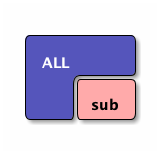
\includegraphics[width=.9\linewidth]{blue.png}
\end{center}
\end{document}
